\documentclass[a4paper,10pt]{article}

\usepackage[english]{babel}
\usepackage[utf8x]{inputenc}
\usepackage{graphicx}
\usepackage{hyperref}
\usepackage{lrec2006}

\title{The Cross-Linguistic Linked Data project}
\name{Robert Forkel}
\address{Max Planck Institute for Evolutionary Anthropology\\ Deutscher Platz 6, D-04103 Leipzig\\ % Your institution
robert\_forkel@eva.mpg.de}

\abstract{The \em{Cross-Linguistic Linked Data} project (CLLD -- \url{http://clld.org}) helps record the world's language diversity heritage
by establishing an interoperable data publishing infrastructure.
I describe the project and the environment it operates in,
with an emphasis on the datasets that are published within the project.
The publishing infrastructure is built upon a custom software
stack -- the \texttt{clld} framework -- which is described next. I then proceed to explain
how Linked Data plays an important role in the strategy regarding interoperability and sustainability.
Finally I gauge the impact the project may have on its environment.\\ \newline \Keywords{Linked Data, Linguistics, Software, Typology}}

\begin{document}
\maketitleabstract

\section{Cross-Linguistic data -- the status quo}
For the purposes of this paper I define cross-linguistic data as either data on many languages, 
or as data about under-resourced languages. I also restrict it to textual data.\footnote{There does not seem to be much of a
Linked Data story for multimedia content anyway.}
Thus, this data will mostly come in the form of 
wordlists, dictionaries, phoneme inventories, typological surveys, small collections of glossed text, grammars, or bibliographies.

This kind of data is the result or forms the basis of much of the work being done at the
department of linguistics of the Max Planck Institute for Evolutionary Anthropology (MPI EVA) in Leipzig which is
one of the centers of what may be called ``language diversity research''.

Since data collection via fieldwork is well respected in this community
%-- writing a grammar seems to be almost like rites of passage
%for becoming a serious linguist -- 
there is not a shortage of data;
often this data is not very complex but even more often it is unpublished. And even if this data is published, it may have ended up as a printed grammar or dictionary,\footnote{Publishing printed grammars and dictionaries seems to get more and more difficult, though~\cite{dlc631}.} which -- given the fact that these are reference works -- is clearly inferior to a digital medium.\footnote{Re-publication or aggregation of data from printed media in digital form is fraught with all the license and copyright issues and the interpretations thereof in the community~\cite{austin2011}.}

Similar observations can be made for typological databases. While many presentations at ALT 10\footnote{The 10th Biennial Conference of the Association for Linguistic Typology, Leipzig August 2013} used data from WALS\footnote{The World Atlas of Language Structures} and complemented it with the author's own data, typically this complementary data is not published.

So there is quite a bit of seemingly low-hanging fruit out there: simple data waiting to get published.

\section{The CLLD project}
\emph{Cross-Linguistic Linked Data} (CLLD) is a project funded by the Max Planck Society for four years, 
setting out to pick this fruit by establishing data publishing infrastructure.

We try to do so by:
\begin{itemize}
\item closing the gap between data creation and data publication by making publication easy and attractive,
% elaborate on recognition thing!? here or below for the journals
\item overcoming the disconnect between data creators and data consumers,\footnote{It is an
interesting observation that at ALT 10 the typical presenters of papers working with
quantitative methods on linguistic datasets were disjoint from the people creating such databases.}
% the common API thing plus the data aggregation aspect!!
\item providing the infrastructure in a sustainable way.
\end{itemize}
% TODO: link to presentation about this Maury guy!

\subsection{The datasets}
Most datasets under consideration right now
have been compiled by or in association with the department of linguistics at the MPI EVA:
\begin{description}
\item[WALS] The \href{http://wals.info}{World Atlas of Language Structures} is now online in its third implementation.
\item[APiCS] The \href{http://apics-online.info}{Atlas of Pidgin and Creole Language Structures} is a typological database modeled after WALS but focussing on pidgins and creoles.
\item[ASJP] (to be published in 2014) \href{http://wwwstaff.eva.mpg.de/~wichmann/ASJPHomePage.htm}{The Automated Similarity Judgement Program} has collected almost 7000 small wordlists of languages and varieties from all over the world.
\item[IDS] (to be published in 2014) The Intercontinental Dictionary Series is a collection of extensive wordlists (ca.~1300 items)
collected for a curated set of meanings covering more than 220 languages.
\item[AfBo] \href{http://afbo.info/}{A world-wide survey of affix borrowing} describes 101 cases of affix borrowing from one language into another.
\item[WOLD] \href{http://wold.livingsources.org}{The World Loanword Database} contains extensive vocabularies (similar to IDS) for 41 languages annotated for loanword status and source words~\cite{tadmor2009}.
\item[Glottolog] \href{http://glottolog.org}{Glottolog} is a language catalog and bibliographical database, comprising close to 8000 languages and more than 200000 bibliographical records~\cite{nordhoff2012}.
\end{description}

But CLLD also provides infrastructure to publish datasets originating outside the MPI EVA:
\begin{itemize}
\item Two data journals (one for dictionaries and one for typological databases) will be started
in 2014 which are open to submissions. These journals will serve the double purpose of
\begin{itemize}
\item allowing publication of datasets referenced in ``traditional'' publications (as is
increasingly required by funders),
\item applying the traditional model of peer-reviewed publications to data, thereby incentivizing
researchers through recognition.
\end{itemize}
\item Bigger datasets can become part of CLLD following an ``edited series'' publication model.
There are already two datasets in this category:
\begin{description}
\item[eWAVE] The electronic \href{http://ewave-atlas.org/}{World Atlas of Varieties of English} is
a typological database containing information on 76 varieties of English.\footnote{Datasets like
eWAVE highlight the fact that ISO 639-3 is not sufficient to identify language varieties.}
\item[PHOIBLE] (to be published in 2014) \href{http://phoible.org}{The Phonetics Information Base}
is a large collection of phoneme inventories for languages from all over the world.
\end{description}
\item Last but not least the \texttt{clld} framework,\footnote{\url{https://github.com/clld/clld}}
upon which all publications are built, is open source software and can be freely reused; i.e.~institutions
or individuals can build applications based on the \texttt{clld} framework to host and publish their own databases.
\end{itemize}

\subsection{The \texttt{clld} framework}
Recognizing that the field of interoperable linguistic data publication is still in its
beginnings\footnote{Although this may have been so for almost 10 years.} adaptability and in general an
iterative approach is called for. Thus, we aim to ``standardize'' on a lower
level, namely on the publication platform; in doing so we hope to make published
resources -- i.e.~the interface to the data -- more adaptable.%\footnote{This may be called the
%"microsoft model" for standardization and clearly has its disadvantages in case we don't stick to "don't be evil".}
\footnote{It should be noted that this is not the first attempt at standardization of a software stack for cross-linguistic databases \cite{dimitriadis2002}; but today's options for community driven development of open source software promise to make a real difference.}
So our aim is at the same time more modest than
semantic interoperability and more ambitious, because the platform is open to serving non-RDF serializations
of resources should these become de-facto standards.

In the first year of the project\footnote{\url{http://clld.org/2014/01/03/new-year.html}} a cross-linguistic database framework -- the \texttt{clld} framework\footnote{Spelled in lowercase conforming to common rules for names of Python software packages} -- has been
developed, which will be the focus of the following sections.
Publishing datasets as \texttt{clld} applications should be seen as a perfect basis for publishing it as Linked Data while at the same time publishing it in a more traditional way (with respect to Web-publishing). It is also a good way to extend the uniformity of the interface from the machine readable data to the user interface accessed with the browser.
While I understand the strength of the Linked Data approach to publishing, being able to also put an attractive human user interface on top of a dataset must not be underestimated when it comes to convincing linguists to open up their data.
Thus the \texttt{clld} framework provides
\begin{itemize}
\item a common core data model,
\item a basic API built on Linked Data principles
\item and what could be termed a ``reference implementation'' of a dataset browser as user-friendly
interface for humans.
\end{itemize}

%I also want to stress that sustainable and maintainable infrastructure has not been a strong point of Linked Data efforts in the past.


\subsubsection{The data model}
\label{sec:datamodel}

The design of the data model was guided by three principles:
\begin{enumerate}
\item All the target datasets have to ``fit in'' without loss.
\item The data model must be as abstract as necessary, as concrete as possible.
\item The data model must be extensible.
\end{enumerate}

Note that these guidelines mirror the requirements set forth in Section 6.1 of \newcite{dimitriadis2002}
for a \emph{linguistic ``metalanguage''}, ensuring unified access to typological databases.
It turns out that most of the datasets we encountered thus far can be modeled using the
following concepts.\footnote{Or as \newcite{burs} put it (further corroborating our experience):
``survey databases are all alike''.}

%
% http://languagelink.let.uu.nl/burs/docs/burs-design.pdf
% Dimitriades. Similar ideas about data model and use cases,
% we focus on publication, though, but want to avoid the "display cabinet" status.
%

\begin{description}
\item[Dataset] holds metadata about a dataset like license and publisher information.
\item[Language] often rather a languoid in the sense of \newcite{dlc623}.
\item[Parameter] a feature that can be coded or determined for a language
-- e.g. a word meaning, or a typological feature.
\item[ValueSet] set of values measured/observed/recorded for one language and one parameter,
i.e. the points in the Language-Parameter-matrix.
\item[Value] a single measurement (different scales can be modeled using custom attributes).\footnote{The only assumption
the core data model makes about values is that they have a name, i.e. a textual description;
datatypes for values can be implemented as application-specific extensions of this core model.}
\item[Unit] parts of a language system that are annotated, such as sounds, words or constructions.
\item[UnitParameter] a feature that can be determined for a unit.
\item[UnitValue] measurement for one unit and one unitparameter.
\item[Source] pointer to secondary literature -- e.g.~bibliographical records.
\item[Sentence] a small piece of text, preferably in the form of interlinear glossed
text\footnote{\url{http://en.wikipedia.org/wiki/Interlinear\_gloss}} according to the
Leipzig Glossing Rules.\footnote{\url{http://www.eva.mpg.de/lingua/resources/glossing-rules.php}}
\item[Contribution] a collection of ValueSets that share provenance information, e.g. authorship.\footnote{Thus,
a CLLD dataset is similar to an edited volume in that it may aggregate data from multiple contributors.}
\end{description}

The relations between these entities are shown in Figure~\ref{cllddatamodel}. Note that
Dimitriadis' \emph{Construction} maps to our \emph{Unit} and \emph{Example} to \emph{Sentence}~\cite[p.~15]{burs}.

\begin{figure}[h!]
  \caption{Entity-relationship diagram of the CLLD core data model}
  \centering
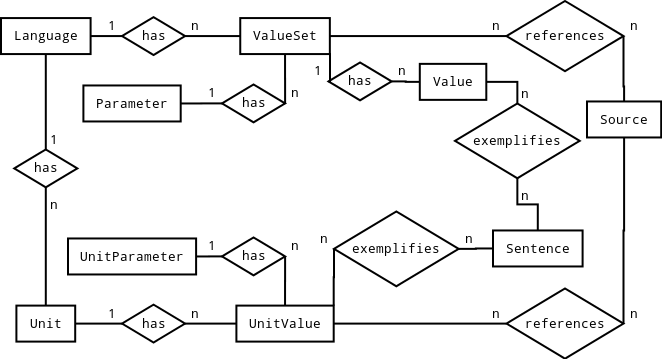
\includegraphics[width=8cm]{clld_erd.png}
\label{cllddatamodel}
\end{figure}

In a concrete incarnation this core data model can be interpreted as shown in Figure~\ref{wolddatamodel}.
Note the additional relation between \emph{Word} and \emph{Counterpart} which is not present in the core model.
The \texttt{clld} framework uses the \emph{joined table inheritance} feature of the \texttt{SQLAlchemy} package
to transparently add attributes to entities of the core data model. 
(see section~\ref{sec:implementation}).\footnote{It should be noted that this data model provides
sufficient structure to allow conversion to the RDF model for wordlists proposed by
\newcite{good2010}.}


\begin{figure}[h!]
  \caption{Entity-relationship diagram of the WOLD data model; \textit{SynSet}s are sets of synonyms,
  a \textit{Counterpart} is an instance of the many-to-many relation between Words and Meanings
  in the sense of \newcite{tadmor2009}.\vspace{0.3cm}}
  \centering
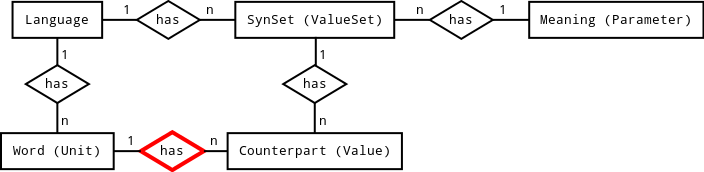
\includegraphics[width=8cm]{wold_erd.png}
\label{wolddatamodel}
\end{figure}


\subsubsection{The implementation}
\label{sec:implementation}
CLLD applications are implemented using the \texttt{clld} framework.\footnote{\url{https://github.com/clld/clld}}
This framework in turn is based on the python packages \texttt{pyramid} and \texttt{SQLAlchemy}
and allows building web applications accessing a relational database.
Using an RDF graph database as main storage was out of the question because of its non-standard requirements
in terms of deployment, administration and maintenance, which would conflict with the strategy
for sustainability described in section~\ref{sec:sustainability}

These technology choices offer the following two essential mechanisms for extensibility:
\begin{enumerate}
\item The joined table inheritance\footnote{\url{http://docs.sqlalchemy.org/en/latest/orm/inheritance.html}}
model provided with \texttt{SQLAlchemy} allows for transparent extension of core database entities.
For each core entity a \texttt{clld} application may define an extended entitity, adding attributes and relations.
Accessing the database using \texttt{SQLAlchemy} makes sure
that whenever the core entitity is queried an instance of the extended entity is returned.
\item The Zope component architecture\footnote{\url{http://www.muthukadan.net/docs/zca.html}}
within pyramid\footnote{\url{http://docs.pylonsproject.org/projects/pyramid/en/latest/narr/zca.html}}
provides an implementation of concepts like interface and adapter, which in turn make it possible to provide
default behavior for entities which works with extended entities as well and can easily be overridden
by registering custom behavior.
\end{enumerate}

Using these mechanisms deviations in terms of data model or user interface are possible, but the
default behavior\footnote{By default, each resource class comes with a list view and a detailed view
for each instance, which in turn can be serialized in various formats like JSON, RDF+XML, etc.}
should be good enough most of the time (at least for the data consumed by machines only).

\subsection{Sustainability: The idea of graceful degradation of service}
\label{sec:sustainability}
Lacking longterm institutional/financial support, a project may employ several methods to gain sustainability:
\begin{enumerate}
\item Make fundraising part of the project activities.
\item Make transfer of ownership easy.
\end{enumerate}

With respect to the CLLD databases the latter means that we always have to take into
consideration what running such a service entails. From our own experience it seems
clear that running interactive web applications without the ability to further develop
the software will lead to dysfunctional applications quickly (within a few years).

But since this scenario is not unlikely in the event of a transfer of ownership, we would
like to define a more stable, and more easily maintainable level of service for our
applications. Thus, we use the Linked Data principles to define a lowest level of service we
want to guarantee for CLLD applications. Doing so means that running CLLD applications can
be as cheap as hosting static files on a web server (and possibly keeping domain
registrations valid).

Essentially we are following the Linked Data principles to provide a REST API for our
datasets that is easy to maintain. Notably, this API is already used today by search engines,
so this aspect of the service will survive also in the lowest level. This also means that
we hope \emph{sustainable operability} as defined by \newcite{dimitriadis2008} can be
provided on top of the Linked Data stack, in particular on top of public sparql endpoints.
Thus, we propose Linked Data to serve as the \emph{Integrated Data and Documentation Format}
described in \newcite{dimitriadis2008} with the additional benefit of a well-defined access protocol.

The \texttt{clld} framework will provide an ``emergency exit'' feature, which will create
a set of files (corresponding to the list and detailed views in various formats as described
above) in an appropriate directory structure to be put on a vanilla webserver.
This can be done by enumerating the resource types, instances and available representations.

%application of linked data as lowest level of service in a graceful degradation of service strategy.
%-> hightlight the API/data access aspect of Linked Data (as opposed to the data model aspect of RDF)

So while Linked Data is still not the way many researchers interested in our datasets\footnote{Most of
the datasets under consideration here are more interesting for typologists than for computational
linguists.}
actually do or want to access data (at least if they can get away with csv instead), there is
something to be gained for the
developer: A stable API across phases of deployment which can be used by any additional services
built on top of the data.


\subsection{Linked Data}

As described above, Linked Data plays an important role in the strategy of the CLLD project.
In the following sections I describe our design choices regarding the implementation of Linked
Data principles for the publication of CLLD datasets.

% TODO: interoperability - merging of distributed resources is a use case Linked Data was invented for!

\subsubsection{URLs and resources}
We do not distinguish \emph{things} from \emph{Web documents} as recommended by \newcite{cooluris},
because the solutions to achieve this conflict with our requirements for easy hosting of the lowest level
of service outlined in section~\ref{sec:sustainability}
These conflicts are also echoed in the list of practical limitations given~\newcite{tennison2011}.
Arguably, using a concept of languages as sets of doculects (following \newcite{dlc623}), the \emph{thing} can
to some extent be identified with the web document describing it anyway;
additionally we rely on the discoverability of context in the sense of \newcite{ambiguity},
e.g.~provided by RDF types or identifiers, to support disambiguation.
%(which is the opposite solution to the one proposed in \newcite{ambiguity}.
%http://www.ibiblio.org/hhalpin/homepage/publications/indefenseofambiguity.html "In defense of ambiguity").
%    see also http://www.jenitennison.com/blog/node/159 What Do URIs Mean Anyway? (Jeni Tennison)

While each RDF resource in CLLD datasets links to its originating
dataset, and this dataset is described by a VoID description (see below), perhaps the most
important bit of provenance information is the domain part of
a resource's identifying URL.\footnote{Since CLLD datasets can be aggregations of multiple
contributions, additional -- more fine grained -- provenance information is typically available,
but for purposes of quality assessment the overriding factor will often be the fact that a
ValueSet is part of an aggregation compiled under editorial control.} Each dataset can employ
additional schemes of conveying additional provenance information, though, like adding a version history.
It is an explicit goal of the project to keep the resource URLs stable and resolvable for
as long as possible, thus, we intend our URLs to be ``cool'' in the old sense, too, and more
generally to fulfill the ``social contract'' between publisher and user outlined in \newcite{ldbp}.

All entities in the clld data model (see section~\ref{sec:datamodel}) map to resource types
in the RDF formulation of this model. Since all entities have a local identifier, a name
and a description, and each CLLD dataset is served from a distinct domain,
we already have all the pieces necessary to fulfill basic requirements for RDF
descriptions.\footnote{e.g. as specified for bio2rdf in its
RDFization-Guide\footnote{https://github.com/bio2rdf/bio2rdf-scripts/wiki/RDFization-Guide}}

\subsubsection{VoID}
\label{sec:void}
The \texttt{clld} framework provides a VoID dataset description for each dataset. This description is populated from
the metadata specified for the dataset, but also using the knowledge the framework has about its entities and capabilities.
E.g. the VoID description for Glottolog\footnote{http://glottolog.org/void.ttl} describes
partitions of the dataset into entitity-type specific subsets (\texttt{void:Dataset}),
and points to data dumps for these, because the number of resources would make accessing
the data via crawling (while still possible) time consuming.

The VoID description and the backlinks of each resource to the dataset are used to provide
provenance and license information for each resource. Following the recommendations for
deploying VoID descriptions in~\newcite{void}, the description is available at the path
\texttt{/void.ttl} of \texttt{clld} applications as well as via content negotiation at the base URL.


\subsubsection{HTTP}

% TODO: intro: we want to highlight the uniform-access aspects of linked data, and these
% pretty much built on features of HTTP

The \texttt{clld} framework uses content negotiation %(see figure~\ref{fig:conneg})
to make sure that RDF resources can be accessed right now just as they would in the ``plain file on webserver'' scenario.
%\begin{figure}
%\label{fig:conneg}
%\caption{HTTP response headers for a resource request with and without explicit \texttt{Accept} header.}
%{\scriptsize
%\begin{verbatim}
%~$ curl -I
%   http://glottolog.org/resource/languoid/id/tomo1245
%HTTP/1.1 200 OK
%Content-Type: text/html; charset=utf-8
%\end{verbatim}
%}

%{\scriptsize
%\begin{verbatim}
%~$ curl -I -H "accept: application/rdf+xml"
%   http://glottolog.org/resource/languoid/id/tomo1245
%HTTP/1.1 200 OK
%Content-Type: application/rdf+xml; charset=utf-8
%\end{verbatim}
%}
%\end{figure}
HTTP link headers are used to identify canonical URLs and alternative representations. %(see figure~\ref{fig:linkheader}).
%\begin{figure}
%\label{fig:linkheader}
%\caption{HTTP \texttt{Link} header returned for a resource request.}
%{\scriptsize
%\begin{verbatim}
%~$ curl -I
%   http://glottolog.org/resource/languoid/id/stan1295
%HTTP/1.1 200 OK
%...
%Link: <http://glottolog.org/resource/languoid
%       /id/stan1295.html>;
%rel="alternate"; type="text/html"
%Link: <http://glottolog.org/resource/languoid
%       /id/stan1295.rdf>;
%rel="alternate"; type="application/rdf+xml"
%...
%
%~$ curl -I
%   http://glottolog.org/resource/languoid
%   /id/stan1295.rdf
%HTTP/1.1 200 OK
%...
%Link: <http://glottolog.org/resource/languoid
%       /id/stan1295>;
%rel="canonical"; type="text/html"
%\end{verbatim}
%}
%\end{figure}
While this feature might not survive in the lowest level of service (unless some custom
webserver configuration is added), it shows the capability of the framework to enumerate
the URL space of its resource graph.


\subsubsection{Linking with other resources and vocabularies}

Linking to resources outside the CLLD universe is clearly in need of further investigation.
Linking to dbpedia and lexvo based on ISO 639-3 codes of languages is possible.
Linking sources to bibliographical records e.g.~in WorldCat is hampered by the fact that
identification of matching records is error prone and not doable ``by hand'' for our typical
source collections with more than 1000 records.

It should be noted, though, that some of our datasets carry the potential to serve as hubs
in the Linked Data cloud themselves, and do so within the CLLD sub-cloud:
\begin{itemize}
\item Glottolog as language catalog and comprehensive bibliography. The desirability of
alternative language catalogs (in addition to Ethnologue or ISO 639-3) is described in
\newcite{dlc610} and can easily be seen looking at a dataset like eWAVE or APiCS, where
many of the languages under investigation are not included in either Ethnologue or ISO-639-3.
\item IDS and WOLD as providers of semi-standard comparison meanings for the
creation of wordlists, i.e. as ``concepticons'' in the sense of \newcite{good2010}.\footnote{It
would probably make sense to link these meanings to wordnet wordsenses but it seems difficult
to determine authoritative URLs for these.}
\end{itemize}


\label{sec:vocab}

While the comprehensive ambition of the CLLD project might warrant the creation of a CLLD
ontology, we have refrained from creating one. This is in large part due to the lack of use
cases (evidenced by lack of usage) for the RDF data.

In an environment where the preferred data exchange format is still csv, I did not want to
venture on an undertaking that might leave us with a bunch of vocabulary URLs to maintain
which no one uses.
Thus, CLLD's current RDF model reuses fairly generic terms from the most common
vocabularies: \texttt{dcterms}, \texttt{skos}, \texttt{foaf}, \texttt{wgs84}.
Due to the extensible architecture provided by the \texttt{clld} framework described in
section~\ref{sec:implementation} each CLLD application is in complete control of the RDF
graphs of its entities, though.\footnote{E.g.~in WALS chapters carry information on the
corresponding linguistic field which often can be linked to dbpedia; WALS languages can be
linked via \texttt{dcterms:spatial} relations to geonames.org countries.}


%\subsection{Linked Data without ontology?}


%- as exemplified many times: RDF does not solve the hosting problem. Linked Data may help, though.
%- as should be clear from above: we stress the publication and unified access aspect of linked data.
%- globally unique identifiers, too -> post-hoc integration see "Distributed Publication and Querying"
%- RDF to us is mainly important, because we can be confident to get all our data into it somehow.


%the best rdf model is not the best (relational) database model. (e.g. GOLD, ...)
%- apart from the question of URLs, defining the RDF datamodel lateron seems a good pragmatic approach.

%So to some extent we are victims of the disconnect between data creators and data consumers ourselves; but then again, having the framework in place will allow adapting to emerging standards easily.

%provenance and data quality asessments:
%For the time being, provenance and quality assessment is something done by the human researcher, because too much context is required.
%In this scenario the two mechanisms to filter data
%- collect all resources of type wordnet:meaning somehow filtered by provenance
%- collect all resources of type Parameter from the datasets IDS, WOLD, ...
%seem equivalent in the amount of context necessary to formulate the queries: In the first case, one must know the wordnet ontology and
%how provenance is conveyed in the data at hand; in the latter one must know that meanings in CLLD lexical databases have type Parameter.


\section{Where does this get us?}

With WALS, APiCS, WOLD, Glottolog and some more datasets\footnote{\url{http://clld.org/datasets.html}}
already published as CLLD applications -- i.e.~with their data available as Linked Data described
via VoID -- I will try to gauge the impact of the CLLD project looking at some use cases:
\begin{itemize}
\item At the most basic level,
fulfilling the request ``give me all you have on language x'' (where x is chosen from one of
the supported language catalogs)
should be possible -- using a local triplestore filled by harvesting the CLLD apps individually
or at a later stage using the CLLD portal.\footnote{Cf. \url{http://portal.clld.org/?q=english}}
\item Testing the conjecture mentioned in WALS chapter "Hand and Arm" \cite{wals-129}
\begin{quote}
The presence of tailored clothing covering the arms greatly increases the distinctiveness of
arm parts and renders more likely their labeling by separate terms [...]. Another potentially
fruitful investigatory strategy would be to cross-tabulate values against the tailoring
technologies of peoples who speak each of the 620 languages of the sample - an enormous
research effort this author must leave to future investigators.
\end{quote}
can still not be done fully automatically, but it should be possible to connect languages
to descriptions about their speakers via dbpedia and start from there.\footnote{If a large,
curated database like \href{http://www.yale.edu/hraf/}{eHRAF} were part of Linked Open Data
this could be possible, though. It should also be noted that cultures, thus anthropological
data, are often identified/distinguished by their language, so that this kind of data
would also fit into the CLLD framework.}
\item Seeding/expanding datasets like ``Tea''~\cite{wals-138}\footnote{This dataset lists for many
languages whether the corresponding word for ``tea'' is derived from Sinitic ``cha'' or
Min Nan Chinese ``te''.}
with data from lexical databases like WOLD\footnote{\url{http://wold.livingsources.org/meaning/23-9}
 lists counterparts for ``tea'' in various languages including their loanword status.}
is already possible.
% thus the cycle of primary data -> derived data can start
\end{itemize}

Arguably, in particular for the case of typological datasets, completely automated use is
still far off.\footnote{Judging by our experience with making
APiCS and WALS structure sets comparable (where APiCS was created with comparability to WALS as an explicit goal),
and evidence provided by \newcite{round2013} at ALT 10 for the difficulty of designing comparable datasets,
it seems clear that ``know your data'' will remain an obligation of the researcher that cannot be shifted to the machine.}
The typical process for analysis of typological datasets will remain a sequence of 
data download, manual inspection, massaging the data, then running analysis software; for this
workflow, the uniform access aspect of Linked Data is the most important.

Thus, the future plans for the project focus on
\begin{itemize}
\item aggregators or portals:
  \begin{description}
  \item[Lexicalia] the portal to lexical data in CLLD datasets\footnote{\url{http://portal.clld.org/lexicalia}} and
  \item[CrossGram] the portal to typological data in CLLD datasets\footnote{\url{http://portal.clld.org/crossgram}}
  \end{description}
  are already under way. In general we would like to follow the example of \href{http://bio2rdf.org}{bio2rdf}
  in providing a standard, versioned, curated aggregation of linguistic data around which a
  community can grow and share analyses, methods and data.
\item ``curated triplestores'' and ``on-demand triplestores'' in the sense of \newcite{tennison2010}.\footnote{Imagine a service that would allow one to:
1. collect a custom dataset from selected features from WALS, APiCS and eWAVE;
2. post-process it with software from CLLD's community repository;
3. dump it in virtuoso and package the appliance as Amazon EC2 AMI ...
}
  On-demand triplestores also look like a good way to go forward with reproducible research\footnote{\url{http://languagelog.ldc.upenn.edu/nll/?p=830}}
  without putting the burden of versioning on each database:
  one will not be able to simply publish a sparql query and the URL of the endpoint, but would have to deposit the triples as well.
\end{itemize}

%
% TODO: this is where there may be overlap with CLARIN, because there may be services in the
% sense of CLARIN involved. Otherwise our aim is - due to all our data being freely available -
% more integration with the web at large.
% - register datasets - fine grained
% - built service that allows sparql-queries on pre-loaded triplestores
% since this may become computationally rather intensive, offering it as limited/restricted
% web service may make sense.
%
For these objectives of the project integration with the CLARIN\footnote{\url{http://clarin.eu}}
infrastructure could be useful.
While the basic data collection and publishing aims more at integration with the web at large,
providing computationally intensive expert services like custom triplestores would profit from
an environment that allows restricted and limited access by a well defined user community.

\bibliographystyle{lrec2006}
\bibliography{refs}
\end{document}
